\documentclass{alex_hü}

\name{Alexander Helbok}
\course{PS Physik}
\hwnumber{13}


\begin{document}
\renewcommand{\labelenumi}{(\alph{enumi})}


\begin{mybox}{1. Totalreflexion im Aquarium}
	\centering \( n = 1.333 \)
	\tcblower
	\begin{enumerate}
		\item \(  \)
		\begin{flalign*}
			\theta_{\text{crit}} &= \arcsin(\tfrac{1}{n}) &&\\
			\epsilon &= \arcsin(n\sin(90 - \arcsin(\tfrac{1}{n}))) = \arcsin(\sqrt{n^2-1}) = \dl{\ang{68.68}} &&
		\end{flalign*}
	\tcbline
		\item \(  \)
		\begin{flalign*}
			\theta_{\text{crit}} &= \arcsin(\tfrac{1}{n}) &&\\
			n_w\sin(\alpha) &= n\sin(90 - \theta_{\text{crit}}) &&\\
			\epsilon &= \arcsin(n_w\sin(\alpha)) = \arcsin(n\sin(90 - \theta_{\text{crit}})) = \arcsin(\sqrt{n^2-1}) &&
		\end{flalign*}
		\( \epsilon \) does not depend on the refractive index of the glass \\[1em]
		If the light source is fixed \( \epsilon \) depends on the thickness of the glass, as the light has to travel almost the same height (less by \( d\tan(\alpha) \) to be exact) in less distance in order to hit the water inside at the same spot.\\
		However if there is no fixed light source, we can displace the beam parallel (so \( \epsilon \) stays constant) to counter the thickness and therefore d does not influence the angle.
	\tcbline
		\item \( n = 1.501 \)
		\begin{flalign*}
			\theta_{\text{crit}} &= \arcsin(\tfrac{1}{n}) &&\\
			\epsilon &= \arcsin(\sqrt{n^2-1}) = 90 - 27.72\iu &&
		\end{flalign*}
		\( \Rightarrow \) we will not get a total internal reflection in this scenario
	\end{enumerate}
\end{mybox}

\begin{mybox}{2. Brewsterwinkel}
	\centering \(  \)
	\tcblower
	\begin{enumerate}
		\item A dipole antenna emits radiation in all directions, except along the pole axis (along the ends of the antennas). So naturally the least energy is radiated off along the axis of the antenna.
	\tcbline
		\item On a microscopic level we find a lot of electric dipoles (like atoms and molecules) that reach an exited state when hit by a light beam. However they can't reradiate in the same direction as their alignment is fixed with the dipole moment, so they give the radiation off in a different direction.
	\tcbline
		\item \(  \)
		\begin{flalign*}
			\theta_B + \theta_r &= \ang{90} &&\\
			n_1\sin(\theta_B) &= n_2\sin(\theta_r) = n_2\sin(90 - \theta_B) = n_2\cos(\theta_B) &&\\
			\theta_B &= \dl{\arctan(\tfrac{n_2}{n_1})} &&
		\end{flalign*}
	\tcbline
		\item \( n_2 = 1.55 \)
		\begin{flalign*}
			\theta_B &= \arctan(\tfrac{n_2}{n_1}) = \arctan(1.55) = \dl{\ang{57.17}} &&
		\end{flalign*}
	\tcbline
		\item Polarizing glasses use Brewster's Angle to block some of the incoming light (horizontally polarized) to reduce glare on eg. the surface of water
	\end{enumerate}
\end{mybox}

\begin{mybox}{3. Polarisation}
	\centering \(  \)
	\tcblower
	\begin{enumerate}
		\item \(  \)
		\begin{flalign*}
			\Delta\phi &= \dl{\tfrac{2\pi}{\lambda}d(n_a - n_0)} &&	
		\end{flalign*}
	\tcbline
		\item \( \Delta\phi = \pi \)
		\begin{flalign*}
			E_{\perp} &= E_0\sin(\theta)\quad \xRightarrow{\text{after}}\quad E_{\perp} = E_0\sin(\theta + \pi) = -E_0\sin(\theta) &&\\
			E_{\parallel} &= E_0\cos(\theta)\quad \xRightarrow{\text{after}}\quad E_{\parallel} = E_0\cos(\theta) &&\\
%			
		\end{flalign*}
		\begin{multicols}{2}
			\begin{minipage}{0.5\textwidth}
				\hspace{2cm} Before \\[1em]
				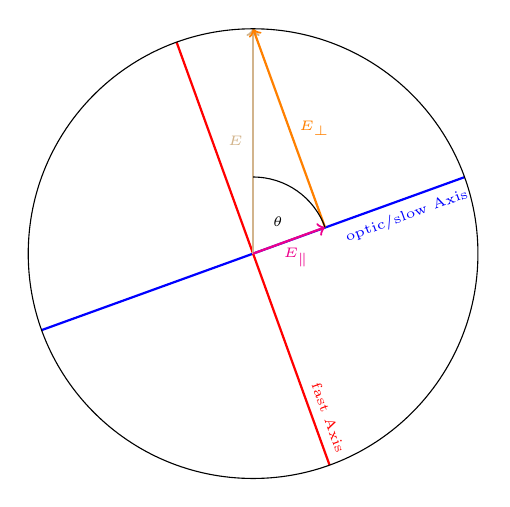
\begin{tikzpicture}
					\begin{axis}[
						width=240pt,
						height=240pt,
						axis lines=none,
						%y axis line style={thick},
						tick align=outside,
						xmin=-1.2,xmax=1.2,ymin=-1.2,ymax=1.2,
						xlabel style={below},
						ylabel style={left},
%						xtick=\empty, ytick=\empty,
%						xticklabels={$-R$, $R$}, yticklabels={\( \tfrac{1}{C\omega} \), \( \omega L \)},
%						xlabel=\tiny optic/slow Axis, ylabel=\tiny fast Axis,
						grid=major,
						grid style={thin,densely dotted,black!20},
						%legend columns=2,
						legend style={at={(axis description cs:0.2,0.2)},anchor=east}]
						\addplot[blue, thick] (-0.94 ,-0.34) -- (0.94 ,0.34) node[below, pos = 0.85,rotate = 20] {\tiny optic/slow Axis};
						\addplot[red, thick] (-0.34 ,0.94) -- (0.34 ,-0.94) node[above, pos = 0.9, rotate = -70] {\tiny fast Axis};
						\addplot[->, Tan, thick] (0,0) -- (0, 1) node [left, pos=0.5] {\tiny$E$};
						\addplot[->, orange, thick] (0.32, 0.117) -- (0, 1) node [right, pos=0.5] {\tiny$E_{\perp}$};
						\addplot[->, magenta, thick] (0,0) -- (0.32, 0.117) node [below, pos=0.6] {\tiny$E_{\parallel}$};
						\draw (0,0) circle (1);
						\draw (0.32,0.117) arc (20:90:0.34);
						\node at (0.11, 0.14) {\tiny$\theta$};
					\end{axis}
				\end{tikzpicture}\\
			\end{minipage}
		\columnbreak
			\begin{minipage}{0.5\textwidth}
				\hspace{2cm} After \\[1em]
				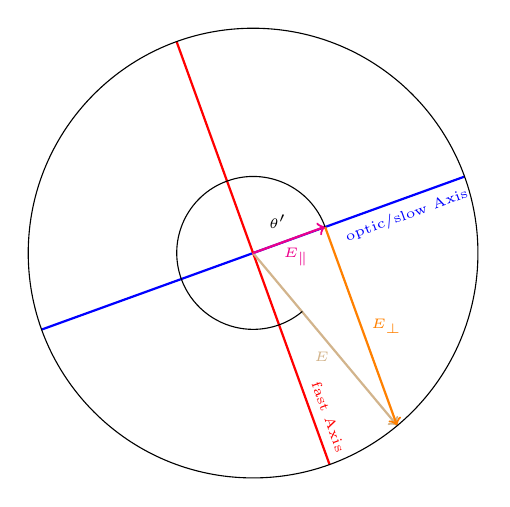
\begin{tikzpicture}
					\begin{axis}[
						width=240pt,
						height=240pt,
						axis lines=none,
						%y axis line style={thick},
						tick align=outside,
						xmin=-1.2,xmax=1.2,ymin=-1.2,ymax=1.2,
						xlabel style={below},
						ylabel style={left},
%						xtick=\empty, ytick=\empty,
%						xticklabels={$-R$, $R$}, yticklabels={\( \tfrac{1}{C\omega} \), \( \omega L \)},
%						xlabel=\tiny optic/slow Axis, ylabel=\tiny fast Axis,
						grid=major,
						grid style={thin,densely dotted,black!20},
						%legend columns=2,
						legend style={at={(axis description cs:0.2,0.2)},anchor=east}]
						\addplot[blue, thick] (-0.94 ,-0.34) -- (0.94 ,0.34) node[below, pos = 0.85,rotate = 20] {\tiny optic/slow Axis};
						\addplot[red, thick] (-0.34 ,0.94) -- (0.34 ,-0.94) node[above, pos = 0.9, rotate = -70] {\tiny fast Axis};
						\addplot[->, Tan, thick] (0,0) -- (0.64, -0.766) node [left, pos=0.6] {\tiny$E$};
						\addplot[->, orange, thick] (0.32, 0.117) -- (0.64, -0.766) node [right, pos=0.5] {\tiny$E_{\perp}$};
						\addplot[->, magenta, thick] (0,0) -- (0.32, 0.117) node [below, pos=0.6] {\tiny$E_{\parallel}$};
						\draw (0,0) circle (1);
						\draw (0.32,0.117) arc (20:310:0.34);
						\node at (0.11, 0.14) {\tiny$\theta'$};
					\end{axis}
				\end{tikzpicture}\\
			\end{minipage}
		\end{multicols}
		\( \theta' = \ang{360} - \theta = \dl{-\theta} \)
	\tcbline
		\item \(  \)
		\begin{flalign*}
			\text{For } \theta &= \ang{0} : \theta' = \dl{\ang{0}} && \\
			\text{For } \theta &= \ang{45} : \theta' = \dl{\ang{315} = \ang{-45}} &&
		\end{flalign*}
	\end{enumerate}
\end{mybox}

\begin{mybox}{4. Physik als Fach}
	\begin{enumerate}
		\item I think Physics both, biased and unbiased. The core thought and motivation behind physics is to get an universal understanding of what goes on around us and in order for this to be universal it has to be unbiased. However the ones doing physics are humans, which frankly speaking suck at being random and unbiased so there will always be a bias due to our human nature. 
	\tcbline
		\item Diversity in Physics is paramount to minimize the bias discussed above because we are all influenced by our background and the more people with different origins work together, the less will the result be biased. A good analogy are random variables that will cancel each other out if they are uncorrelated (a team of different people) and will amplify each other if they are correlated (a team of people with the same ethnic background).
	\tcbline
		\item I don't think all people in the physical community get the same treatment. For example try to name a black physicist. And it gets even harder if we also ask for a nobel prize. In fact this is impossible as to date no nobel prize in science can be attributed to an African American scientist. This is partly due to the fact that less colored children even enroll in a university course in science so naturally less are eligible for a nobel prize but the fact that not a single one has been awarded to them and only three have been awarded to women is simply shocking. 
	\end{enumerate}
\end{mybox}

\end{document}